%Doc config

\documentclass[11pt,letterpaper]{article}

\usepackage{graphicx}
\usepackage{textcmds}
\usepackage[left=3cm,right=3cm,top=3cm,bottom=4cm]{geometry}


\usepackage[
    backend=biber,
    style=apa,
    sortlocale=de_DE,
    natbib=true,
    url=false, 
    doi=true,
    eprint=false
]{biblatex}






%\addbibresource{biblio.bib}

\newcommand{\fontsmall}{\fontsize{7pt}{10pt}\selectfont}
\newcommand{\fontnormal}{\fontsize{11pt}{16pt}\selectfont}
\newcommand{\headline}{\fontsize{17pt}{26pt}\selectfont}

\bibliography{biblio}


\begin{document}


   \title{The Impact of Smartphone Use on Personal Satisfaction} 



\noindent\begin{minipage}{0.5\textwidth}
\fontsmall
Management Center Innsbruck \\
Department Management, Communication \& IT  \\
ILV Digital Behavior


\end{minipage}%
\hfill%
\begin{minipage}{0.3\textwidth}\raggedleft

\includegraphics[height=1.0cm]{mci-logo.png}

\end{minipage}


 
\begin{center}
\textbf{Homework: Digital Behavior}\\   %Title
Florian Bigelmaier\\                         %Name
November, 1st 2021\\                         %Date
\end{center}
\rule{\linewidth}{0.1mm}




\headline \begin{center}
The Impact of Smartphone Use on The Personal Satisfaction and A Personal Experiment
\end{center} 
\fontnormal 
Five hourse every day. This is the amount of time my smartphone reports me as an usual daily display-on time. There is no other interpretation than to asume, that this small device is infleucing my personal life in an tremendous way. As I try to show with some concepts and examples - there are positive aspects and reasons to behave like this. But parallely, being influenced by information technology at such an high level (actually five hours fill almost a third of my active day) has also negative consequences. My personal aim for doing this homework is to come to more conscious decisions and understand my smartphone like a technical instrument, not as an proxy for personal contact as it might appears to be sometimes. As I want to try to reflect on this aim and the process to it, I want to try to formulate this homework in a way that is at least inspired by scientific methodology and standards. Therefore I will switch for the rest of this paper in an objective third person style. When trying to work scientifically it is basically necessary to define a hypothesis that can be validated or neglected. For this paper the hypothesis will be:

\begin{center}
\textit{The personal satisfaction in life increases when the use of the smartphone is limited to conscious usage.}
 \end{center}

This hypothesis is based on two assumptions. First, the smartphones seems to help in the everyday life in several ways. Therefore one assumption is, that the basic use of the smartphone as a tool affects the personal satisfaction positively. Second, unconscious use of the smartphone has no clear generated value or outcome. For example endless scrolling in a social media feed beneath the usual dosis of getting up to date does not seem to have any advantage. Therefore the second assumption is, that unconscious use of the smartphone affects the personal satisfaction in a negative way. Both assumptions are necessary for stating the hypothesis.

\section*{Methodology}
This paper does not follow the standards of scientific methodologies as it is supposed to be a personal reflection. Nevertheless this paper follows a strucuted idea of proving the above mentioned hypothesis. Furthermore, the two assumptions above need to be questioned. The methodology should therefore be open enough to challenge these assumptions as well. 

The evaluation of this hypothesis will be measured by a personal experiment with the duration of three days. From 28th until 30th of October the person will try to use the smartphone in a more conscious way as describe later on. The person will record their personal experience in a diary. 

The dependent variable of the hypothesis is the \textbf{personal satisfaction}. The personal satisfaction is apparently a complex dimension to be measured. In this case it will be tracked by a diary and the subjective impression how conscious decisions regarding the smartphone use affected the feeling of the person in any related manner. Therefore the above mentioned diary contains for each day notes on the following questions:
\begin{enumerate}
\item 
How long and in which manner did you use the smartphone today?

\item
What are your subjective positive and negative thoughts on the use of the smartphone today?

\item
Which non-digital activities were possible due to the smaller amount of smartphone use?

\item
Which digital acitivities did you consciously decide not to do?

\item
How did these conscious decisions (regarding the last two questions) affect your personal satisfaction?

\item
Do you want to add any further personal notes regarding your smartphone use today?

\end{enumerate}

The independent variable that will be manipulated during the experiment are named in the hypothesis as \textbf{conscious usage}. More precisely, the affective decisions of smartphone use will be replaced by a rule based decision making for the first above mentioned interval. The rules will emerge out of an analysis of smartphone use and thoughts and concepts that are presented in the following paragraphs. Therefore they will be formulated later on.

\section*{Context and Concepts: 14 Years Of Change}
\begin{center}
\qq{Mobile is eating the world} \autocite[][]{evans14}
 \end{center}
When Benedict Evans, a former analyst of the U.S. venture capital fonds Andreesen Horrowitz, formulated this statement in 2014 a revolution just had taken place in the seven years before: In 2007 the first iPhone was released and changed the way how people interact with digital systems dramatically without any question. But beneath this, the iPhone and Smartphone brought several aspects with them, that changed even the every day life for their users - i.e. a big part of the worlds population. Just to name two of them: 
\begin{itemize}
\item 
The \textbf{ubiquity} of the mobile tech architecure including smartphones and the cellular access to the internet made it possible to access the internet wherever a demand could exist \autocite[][p.1]{okazaki13}. This is the basis for situations like paying at the grocery store with digital payment method or using the smartphone as a key for a vehicle.
\item
The \textbf{context sensitivity} of mobile devices differentiates them from former devices: Smartphones are not only small computers, they also come with several sensors that allow e.g. to determin the phones location (via GPS)\autocite[][p.1]{minch04}. Other players in the mobile eco system like providers of apps have the possibility to understand the context of the user by using these sensor data and generate a contextualised environment. An example for this might be the localisation of search results in the Google Maps App. When searching for a restaurant, the App will recommend restaurants that are near to the user and are open for guests at the immediate context of the user.
\end{itemize}

Beneath these new opportunities for entrepreneurs to build new businesses and the end users who profit with an increase of convenience, there is also a shady side of this development. In his essay \qq{Is Google Making Us Stupid?}, \cite[][]{carr08} provocately lists several artefacts of this shady side. For this homework, the most important points of this article are the following ones. All of them with no further references or proven empirical validation.
\cite[][]{carr08} points out, that due to several factors, reading online ist faster and more on the surface of the text not least because of a shorter attention span resulting of the big variety in alternatives for information and entertainment that are only one mouse click away. Furthermore he draws an comparison to the invention of the printing machine and the upcoming revolution of cheaper books. The advantages like more education and availability of information for a broader part of the society and the possibility to publish a bigger variety of knowledge came along with disadvantages. Just like the pros, the cons also are comperable with the digital revolution: The lower the burdens are to publish, the lower the trust is in integrity and authentizity of these publications. A third major point which will come up later again in this homework is the brain change, \cite[][]{carr08} refers to. This change is not a kind of neurological mutation. A change can be more likely observated in the orientation of the individuals. When clocks were available, the way how to plan a day shifted from a sun-oriented and gut-feeling-inspired one to a hard orientation after the 24 hours of the day. \cite[][]{carr08} sees this point in the last 14 years as well: In a more abstract way, smartphones changed the way, individuals orient themselves in their construction of their environment.

An alternative point of view is deliverd by \cite{gergen02} and \cite{ward17} who are referring to the concepts of absent presence respectively the cognitive consequences of smartphone use.
\begin{center}
\qq{We are present but simultaneously rendered absent; we have been erased by an absent presence} \autocite[][p.227]{gergen02}
\end{center}
\cite{gergen02} already pointed out in 2002 that the use of modern forms of communication is so immersive, that people do not pay attention to and interact actively with their environment in which they are physically present. \cite{gergen02} is referring to this as a challenge. He states that \qq{The erosion of face-to-face community, a coherent and centered sense of
self, moral bearings, depth of relationship, and the uprooting of meaning from material context [...] are [...] repercussions of absent presence}\autocite[][p.236]{gergen02}. In addition to that, \cite{ward17} researched on the question how the extensive use of smartphones and the integration in the daily live affects the cognitive ressources of humans. In two experiments they could prove, \qq{that the mere presence of consumers’smartphones can adversely affect two measures of cognitive capacity — available
working memory capacity and functional fluid intelligence} \autocite[][]{ward17}. The combined point of view of \cite{gergen02} and \cite{ward17} will be a basis for providing support to the concious decisions to make for the first interval of the experiment.


\section*{Analysis of Smartphone Use}
As a starting point for finding optimizations for more conscious decisions there should be an analysis of the status quo. Therefore especially three questions are of interest. 
\begin{enumerate}
\item How long do you use the smartphone every day?
\item Which sort of acitivity do you use in this time?
\item When are the times where unconscious and non value-adding smartphone use occurs?
\end{enumerate}

\subsection*{1. How Long Do You Use The Smartphone Every Day?}
Regarding the question of total smartphone use, the built in functionality of the person's smartphone (an iPhone XR) for display time analysis has been used as a basis. The row data has been extracted manually. 

\begin{figure}[h]
\centering
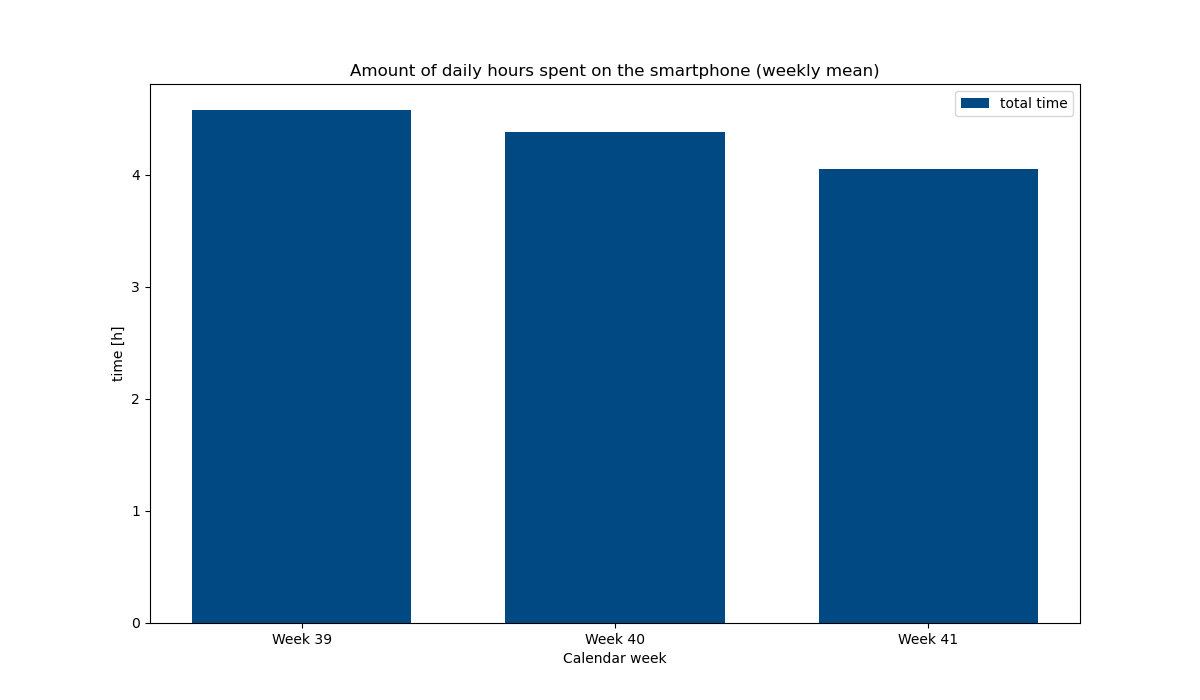
\includegraphics[width = \textwidth]{../data/usage-times-total.png}
\caption{Graph shows weekly average of persons daily display time}
\end{figure}

It can be stated, that the usual daily display time is approximately four hours.

\subsection*{2. Which sort of acitivity do you use in this time?}
To analyse deeper, how the smartphone is used, the used applications and contents have been clustered in four categories. These are the following: Social Media, Instant Messaging, Web Browsers and News and Entertainment. To ensure a proper analysis, this time the total weekly amount of use per category has been chosen as a suitable metric because of variations in the distribution from one weekday to another. The web browsers are a frequently used category as the person uses the browser frequently for streaming radio or television when there is no technical requirement to install an app.

\begin{figure}[h]
\centering
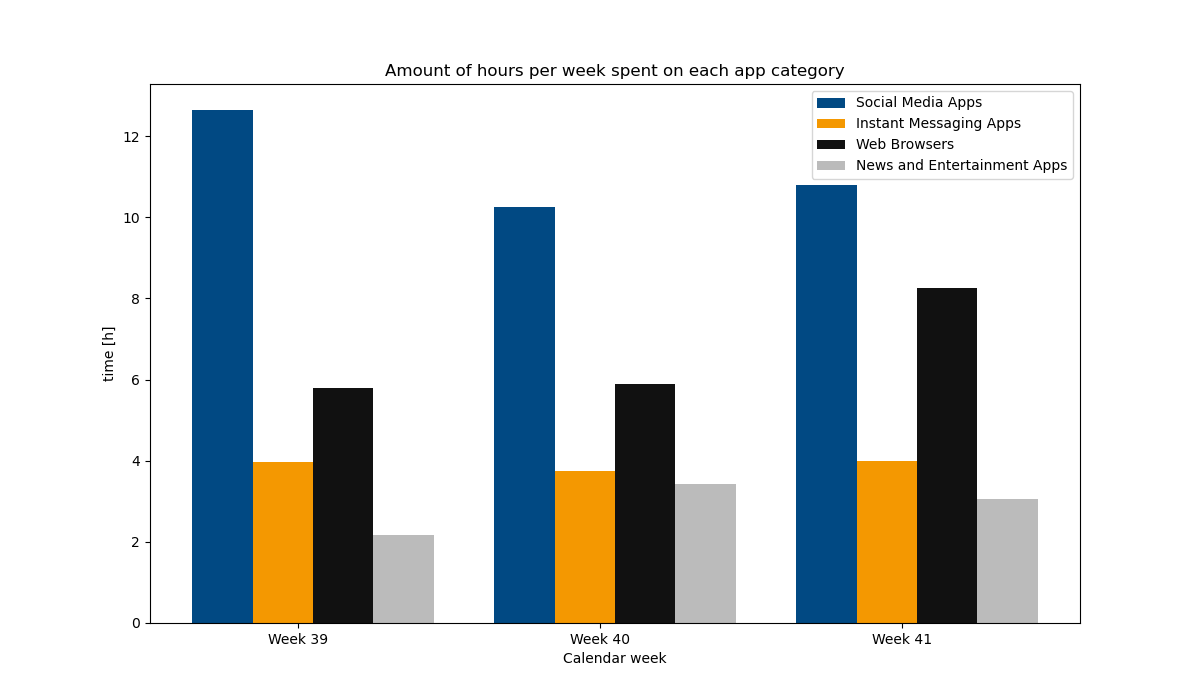
\includegraphics[width = \textwidth]{../data/usage-times.png}
\caption{Graph shows how the evaluated person used the smartphone in the three weeks before the experiment}
\end{figure}

This data set provides several interesting insights. First of all, social media is the category of apps which sums up to the most hours of use. This seems to be an suitable point to question conscious decisions. For the first thought, there is no rational explanation for ten to twelve hours of social media use per week. Furthermore, the browsing is a category with much attributed display time. As a browser is a universal tool to access different types of media and content, there are several browsed sites behind this amount of time. On reason for the high amount of time is the usage for streaming of news like the German \textit{Tagesschau} or the Austrian radio station \textit{Hitradio Ö3}. Together with the news and entertainment section (sums up for two to three hours per week) this could also be a starting point to think about optimized and conscious news consumption. Last, the apps used for Instant Messaging (i.e. \textit{Whatsapp}, \textit{Signal}) have also a high absolute amount of display time around six to eight hours per week.

\subsection*{3. When are the times where unconscious and non value-adding smartphone use occurs?}
This question cannot be resolved in a such easy manner like in the above answered questions as there is no row data nor report from the smartphone itself. Much more this depends on subjective perception of the observed person. In this case there are especially three occasions of unconscious use: First, in the morning right after the ringing of the alarm and before the way to the bathroom and breakfast. Of course, there is a subjective percieved need to inform about messages and information that could have come in the night before, but after this the time is missused for unintended scrolling and browing in social media apps. Second, during the day in focus times (e.g. learning, working etc.) the smartphone seems to be attractive for a quick look even if there is no need for having a look on the smartphone or any trigger like a notification. Third the consumption of news is unstructured and distributed over the whole day, driven by notifications and ocasional opening of news apps like \textit{Der Spiegel} or \textit{Der Standard}.

\section*{Derivating a plan for the experiment}
The aim of this paper is to find out, if there is a correlation between the subjective percepted satisfaction and a more conscious use of the smartphone. Therefore the hypothesis implies that more conscious decisions are to made during a normal day of smartphone use. As seen in the section above, the person uses his smartphone around four hours per day and just based on the interpretation of the smartphone use, there are already several possible starting points for a more efficient and less time-consuming smartphone use. Nevertheless, this hugh amount also shows, that conscious decisions are not possible for every time unlocking the phone. Therefore it is inevitable to work with simple rules which aim to reduce the smartphone use based on the mentioned possible interesting starting points for further exploration. These rules are suitable to reduce the complete unintended use. Anyways, if there is a good reason for the use of the smartphone, a conscious decision can always override these rules.

\textbf{Rule 1: Social Media in the morning}
One obvious point of a possible unconscious and unintend use of the smartphone is the scrolling and browsing in social media apps in the morning. Therefore the rule says, that the person may not use the smartphone before the end of the morning routine including breakfast. \newline

\textbf{Rule 2: Shift browsing to notebook or desktop devices}
One rather hypothetical idea is to reduce the time spent on the mobile browsers by reducing the casual browsing. If there is something interesting to look up, notes should be taken by the person instead of a immediate search on the smartphone which may lead to an unintended browsing after the actual question has been answered. \newline

\textbf{Rule 3: Concentrate news consumption to one period per day}
A further reason for the extensive amount of time spent on the browser and the smartphone in total is to get the latest news in Germany, Austria, the marketing and tech industry and the whole world. As there are seldom news that need to be consumed within hours, it should be enough to consume news once a day in the evening. This allows to focus on the preferred channels but also to investigate further one or two interesting topics in detail and not browse in news apps several times a day superficially. \newline

\textbf{Rule 4: Instant Messaging not in focus times}
Instant Messaging requires instant reading and answering at least if the term is interpreted literally. This requirement is unrealistic but leads to the consequence that the person is checking for messages frequently. On a rational point of view, a look on the smartphone once in two hours during the active working and study times of the day should be enough to answer with an adequate response time. This allows the user to focus on the work and his studies. Therefore the rule should be: Do not use the smartphone during self-set focus time of 30 minutes to two hours in a block. \newline

\section*{Observations during the experiment}

\section*{The effect of conscious usage regarding smartphone use on the personal satisfaction}

\subsection*{Discussion and reflection in combination with the article}

\newpage





\printbibliography 

\end{document}
